\cleardoubleemptypage
\renewcommand*\chapterpagestyle{scrheadings}
\chapter{Results}
The result of the project ended up being a fully operational voice assistant with a hardware frontend and a Rust backend.
The hardware frontend contains a 3D-printed case covering a Raspberry Pi and a 10.1-inch HDMI display;
the Raspberry Pi is powered by either a DC jack or a battery, depending on the users preference ---
this is realized using a custom printed circuit board and a battery management system.
The custom PCB connects to the Raspberry Pi's GPIO pins and provides a more accessible alternative to the displays touchscreen,
that being a recording button, which when pressed, can start or stop the recording of a query,
as well as a wake word switch --- this allows the user to enable or disable wake word detection (and therefore hands-free usage) using a button.
There is also an RGB led on the PCB, which shows different color codes when errors occur, albeit any errors
that occur during processing will be made known to the user via the voice assistant output.

The software backend is implemented in the Rust programming language, picked due to performance and developer ergonomics.
It is built using a microservice architecture, where each part of the program is its own separate microservice trait,
allowing multiple implementations for each microservice and therefore, using the robust configuration system,
the ability to configure each step of the way from an audio input to an output --- be that configuring
a microservice to run locally or remotely, or configuring parameterns, such as if local machine learning models
should be run on the GPU or on the CPU.

The following flowchart demonstrates the architecture, with the backend depicted as the server and the frontend depicted as the client:
\begin{figure}[H]
\centering
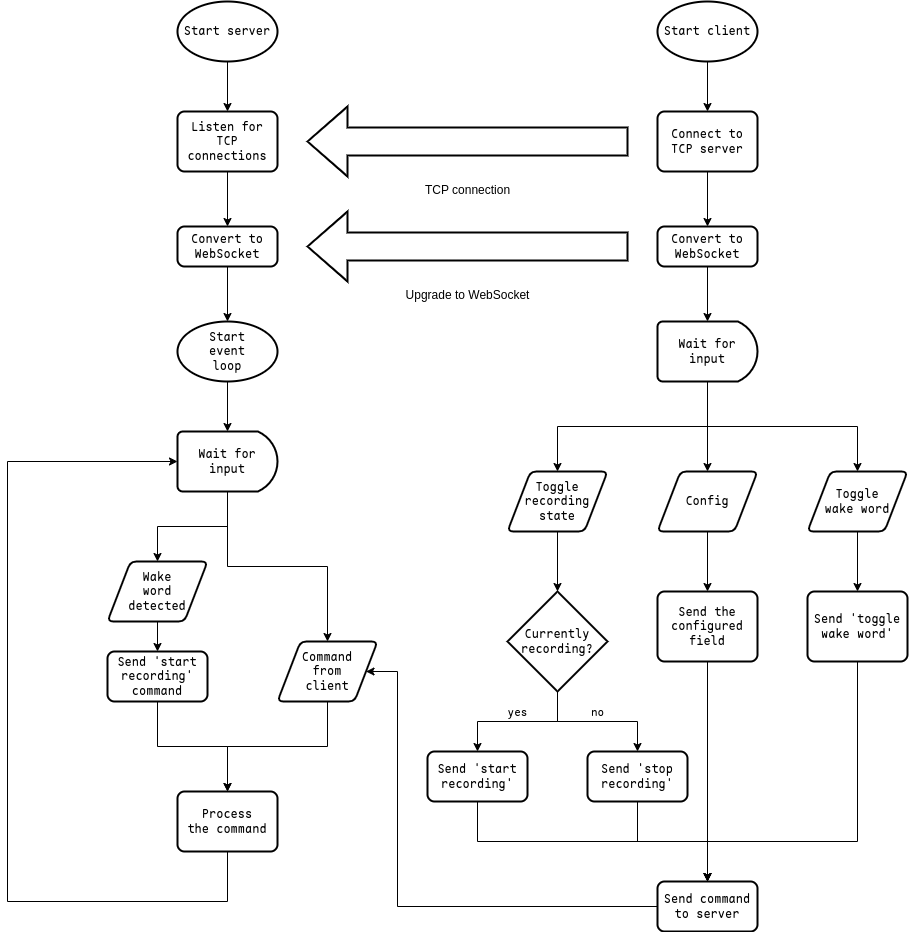
\includegraphics[width=\textwidth]{assets/architecture}
\caption{Client-Server Architecture}
\label{chart:architecture}
\end{figure}

The process starts with the server listening for TCP connections, and a client connecting to the server, immediately after which,
the connection is upgraded to WebSocket.
In the main event loop, the server waits for input from the client, while the client waits for input to the user;
the user can start the recording by pressing the record button, after which the client checks if there is a recording currently running:

\begin{itemize}
    \item If there is no recording active, the client sends a \texttt{start recording} command to the server
    \item If there is a recording active, the client sends a \texttt{stop recording} command to the server
\end{itemize}

another --- arguably much simpler --- way for the user to start the recording is to say the wake word, which the server listens for
using the audio recording microservice.
The user can also configure a setting on the client (in the reference frontend application implementation this is done via the settings menu),
which sends a \texttt{config table.key=value} command to the server, where table, key, and value are some setting that the user configured.
Finally, the user can also toggle wake word detection, which sends a \texttt{toggle wake word} command to the server and either enables or disables
wake word detection.

\section{Final Discussion}
The project can be considered complete --- all required features have been successfully implemented.
Future enhancements could focus on expanding the feature set and improving the user experience when interacting with the frontend.
Moreover the audio recording system should be overhauled, possibly by moving it back to the frontend;
Timers are also not perfect yet, as they do not have a ringtone.
Additional speech-to-text models may also be explored to improve accuracy and response time.

As a note to self for the future:
More extensive testing is a generally a good idea --- testing manually wastes a lot of precious time
and hunting bugs when automated tests could have discovered them automatically should not be necessary.
Usability studies should be conducted to better understand how the system performs in real-world scenarios, while interacting with real users.
